\documentclass[a4]{article}
\pagestyle{myheadings}

%%%%%%%%%%%%%%%%%%%
% Packages/Macros %
%%%%%%%%%%%%%%%%%%%
\usepackage{mathrsfs}


\usepackage{fancyhdr}
\pagestyle{fancy}
\lhead{}
\chead{}
\rhead{}
\lfoot{}
\cfoot{} 
\rfoot{\normalsize\thepage}
\renewcommand{\headrulewidth}{0pt}
\renewcommand{\footrulewidth}{0pt}
\newcommand{\RomanNumeralCaps}[1]
{\MakeUppercase{\romannumeral #1}}

\usepackage{amssymb,latexsym}  % Standard packages
\usepackage[utf8]{inputenc}
\usepackage[russian]{babel}
\usepackage{MnSymbol}
\usepackage{amsmath,amsthm}
\usepackage{indentfirst}
\usepackage{graphicx}%,vmargin}
\usepackage{graphicx}
\graphicspath{{pictures/}} 
\usepackage{verbatim}
\usepackage{color}









\DeclareGraphicsExtensions{.pdf,.png,.jpg}% -- настройка картинок

\usepackage{epigraph} %%% to make inspirational quotes.
\usepackage[all]{xy} %for XyPic'a
\usepackage{color} 
\usepackage{amscd} %для коммутативных диграмм


\newtheorem{Lemma}{Лемма}[section]
\newtheorem{Proposition}{Предложение}[section]
\newtheorem{Theorem}{Теорема}[section]
\newtheorem{Corollary}{Следствие}[section]
\newtheorem{Remark}{Замечание}[section]
\newtheorem{Definition}{Определение}[section]
\newtheorem{Designations}{Обозначение}[section]




%%%%%%%%%%%%%%%%%%%%%%%% 
%Сношение с оглавлением% 
%%%%%%%%%%%%%%%%%%%%%%%% 
\usepackage{tocloft} 
\renewcommand{\cftdotsep}{2} %частота точек
\renewcommand\cftsecleader{\cftdotfill{\cftdotsep}}
\renewcommand{\cfttoctitlefont}{\hspace{0.38\textwidth} \LARGE\bfseries} 
\renewcommand{\cftsecaftersnum}{.}
\renewcommand{\cftsubsecaftersnum}{.}
\renewcommand{\cftbeforetoctitleskip}{-1em} 
\renewcommand{\cftaftertoctitle}{\mbox{}\hfill \\ \mbox{}\hfill{\footnotesize Стр.}\vspace{-0.5em}} 
\renewcommand{\cftsubsecfont}{\hspace{1pt}} 
\renewcommand{\cftparskip}{3mm} %определяет величину отступа в оглавлении
\setcounter{tocdepth}{5} 




\addtolength{\textwidth}{0.7in}
\textheight=630pt
\addtolength{\evensidemargin}{-0.4in}
\addtolength{\oddsidemargin}{-0.4in}
\addtolength{\topmargin}{-0.4in}

\newcommand{\empline}{\mbox{}\newline} 
\newcommand{\likechapterheading}[1]{ 
	\begin{center} 
		\textbf{\MakeUppercase{#1}} 
	\end{center} 
	\empline} 

\makeatletter 
\renewcommand{\@dotsep}{2} 
\newcommand{\l@likechapter}[2]{{\bfseries\@dottedtocline{0}{0pt}{0pt}{#1}{#2}}} 
\makeatother 
\newcommand{\likechapter}[1]{ 
	\likechapterheading{#1} 
	\addcontentsline{toc}{likechapter}{\MakeUppercase{#1}}} 





\usepackage{xcolor}
\usepackage{hyperref}
\definecolor{linkcolor}{HTML}{000000} % цвет ссылок
\definecolor{urlcolor}{HTML}{AA1622} % цвет гиперссылок

\hypersetup{pdfstartview=FitH,  linkcolor=linkcolor,urlcolor=urlcolor, colorlinks=true}



\def \newstr {\medskip \par \noindent} 



\begin{document}
	\def\contentsname{\LARGE{Содержание}}
	\thispagestyle{empty}
	\begin{center} 
		\vspace{2cm} 
		{\Large \sc Санкт-Петербургский Политехнический Университет}\\
		\vspace{2mm}
		{\Large\sc Петра Великого}\\
		\vspace{1cm}
		{\large \sc Институт прикладной математики и механики\\ 
			\vspace{0.5mm}
			\textsc{}}\\ 
		\vspace{0.5mm}
		{\large\sc Кафедра $"$Прикладная математика$"$}\\
		\vspace{15mm}
		
		
		{\sc \textbf{Отчёт\\
			Лабораторная работа №$5-8$\\
			по дисциплине\\
			"Математическая статистика"}
			\vspace{6mm}
			
		}
		\vspace*{2mm}
		
		
		\begin{flushleft}
			\vspace{4cm}
			\sc Выполнил студент:\\
			\sc Салихов С.Р.\\
			\sc группа: 3630102/70401\\
			\vspace{1cm}
			\sc Проверил:\\
			\sc к.ф-м.н., доцент\\
			\sc Баженов Александр Николавич
			\vspace{20mm}
		\end{flushleft}
	\end{center} 
	\begin{center}
		\vfill {\large\textsc{Санкт-Петербург}}\\ 
		2020 г.
	\end{center}
	
	\newpage
	\pagestyle{plain}
	
	%\begin{center}
	%\begin{abstract} 
	
	%\end{abstract}
	
	%\end{center}
	
	\newpage
	\tableofcontents{}
	\newpage
	\listoffigures
	\newpage
	\listoftables
	\newpage
	
	
	\section{Постановка задачи}
		1)Сгенерировать двумерные выборки размерами 20, 60, 100 для нормального двумерного распределения N(x, y, 0, 0, 1, 1, $\rho$).\\
		Коэффициент корреляции $\rho$ взять равным 0, 0.5, 0.9.\\
		Каждая выборка генерируется 1000 раз и для неё вычисляются: среднее значение, среднее значение квадрата и дисперсия коэффициентов корреляции Пирсона, Спирмена и квадрантного коэффициента корреляции.
		Повторить все вычисления для смеси нормальных распределений:

		$$f(x, y) = 0.9N(x, y, 0, 0, 1, 1, 0.9) + 0.1N(x, y, 0, 0, 10, 10, -0.9).$$
		Изобразить сгенерированные точки на плоскости и нарисовать эллипс равновероятности.\\
	
		2)Найти оценки коэффициентов линейной регрессии $y_i = a + bx_i + e_i$, используя 20 точек на отрезке $[-1.8; 2]$ с равномерным шагом равным 0.2. Ошибку $e_i$ считать нормально распределённой с параметрами (0, 1). В качестве эталонной зависимости взять $y_i = 2 + 2x_i + e_i$. При построении оценок коэффициентов использовать два критерия: критерий наименьших квадратов и критерий наименьших модулей. Проделать то же самое для выборки, у которой в значения $y_1$ и $y_20$ вносятся возмущения 10 и -10.\\
		
		3)Сгенерировать выборку объёмом 100 элементов для нормального распределения N(x, 0, 1). По сгенерированной выборке оценить параметры $\mu$ и $\sigma$ нормального закона методом максимального правдоподобия. В качестве основной гипотезы $H_0$ будем считать, что сгенерированное распределение имеет вид N(x, $\hat{\mu}$, $\hat{\sigma}$). Проверить основную гипотезу, используя критерий согласия $\chi^2$. В качестве уровня значимости взять $\alpha$ = 0.05. Привести таблицу вычислений $\chi^2$.\\
		
		4)Для двух выборок размерами 20 и 100 элементов, сгенерированных согласно нормальному закону N(x, 0, 1), для параметров положения и масштаба построить асимптотически нормальные интервальные оценки на основе точечных оценок метода максимального правдоподобия и классические интервальные оценки на основе статистик $\chi^2$ и Стьюдента. В качестве параметра надёжности взять $\gamma$ = 0.95.
	\section{Теория}
		\subsection{Двумерное нормальное распределение}
			Двумерная случайная величина (X, Y) называется распределённой нормально (или просто нормальной), если её плотность вероятности определена
			формулой
			
			$$N(x, y, \overline{x}, \overline{y}, \delta_x, \delta_y, \rho) = \frac{1}{2\pi\delta_x\delta_y\sqrt{1 - \rho^2}} * exp\left\{
			\begin{array}{ccc}
			-\frac{1}{2(1 - \rho^2)} [\frac{(x - \overline{x})^2}{\delta^2_x} - 2\rho\frac{(x - \overline{x})(y - \overline{y})}{\delta_x \delta_y} + \frac{(y - \overline{y})^2}{\delta^2_y}]
			\end{array}
			\right\}$$
			
			Компоненты X, Y двумерной нормальной случайной величины также распределены нормально с математическими ожиданиями x, y и средними квадратическими отклонениями $\delta_x$, $\delta_y$ соответственно. \\
			Параметр $\rho$ называется коэффициентом корреляции.
		
		\subsection{Корреляционный момент(ковариация) и коэффициент корреляции}
			Корреляционным моментом, иначе ковариацией, двух случайных величин X и Y называется математическое ожидание произведения отклонений этих случайных величин от их математических ожиданий.
			
			$$K = cov(X, Y) = M[(X - \overline{x})(Y - \overline{y})]$$
			
			Коэффициентом корреляции $\rho$ двух случайных величин X и Y называется отношение их корреляционного момента к произведению их средних квадратических отклонений:
			$$\rho = \frac{K}{\delta_x\delta_y}$$

			
			Коэффициент корреляции — это нормированная числовая характеристика, являющаяся мерой близости зависимости между случайными величинами
			к линейной.
			
			\subsection{Выборочные коэффициенты корреляции}
				\subsubsection{Выборочный коэффициент корреляции Пирсона}
					
Пусть по выборке значений 
					

					
$\{{x_i, y_i}\}^n_1$ 1 двумерной с.в. (X, Y ) требуется оценить коэффициент корреляции $\rho$ = $\frac{cov(X, Y)}{\sqrt{DX DY}}$. Естественной оценкой для $\rho$ служит его статистический аналог в виде выборочного коэффициента корреляции, предложенного К.Пирсоном, —
					

					
$$r = \frac{\frac{1}{n} \sum(x_i - \overline{x})(y_i - \overline{y})}{\sqrt{\frac{1}{n} \sum (x_i - \overline{x})^2 \frac{1}{n} \sum(y_i - \overline{y})^2})} = \frac{K}{s_X s_Y}$$
					
где K, $s^2_X, s^2_Y$ - выборочные ковариации и дисперсии с.в. X и Y.
					

					
\subsubsection{Выборочный квадрантный коэффициент корреляции}
					
	Кроме выборочного коэффициента корреляции Пирсона, существуют и другие оценки степени взаимосвязи между случайными величинами. К ним относится выборочный квадрантный коэффициент корреляции
					
	$$r_Q = \frac{(n_1 + n_3) - (n_2 + n_4)}{n}$$
					
	
					
	где $n_1, n_2, n_3 и n_4$ - количества точке с координатами $(x_i, y_i)$, попавшими
					
	соответственно в I, II, III и IV квадранты декартовой системы с осями $x' = x - med x, y' = y - med y$ и с центром в точке с координатами (med x, med y).
					
					\subsubsection{Выборочный коэффициент ранговой корреляции Спирмена}
						На практике нередко требуется оценить степень взаимодействия между качественными признаками изучаемого объекта. Качественным называется признак, который нельзя измерить точно, но который позволяет сравнивать изучаемые объекты между собой и располагать их в порядке убывания или возрастания их качества. Для этого объекты выстраиваются в определённом порядке в соответствии с рассматриваемым признаком. Процесс упорядочения называется ранжированием, и каждому члену упорядоченной последовательности объектов присваивается ранг, или порядковый номер. Например, объекту с наименьшим значением признака присваивается ранг 1, следующему за ним объекту — ранг 2, и т.д. Таким образом, происходит сравнение каждого объекта со всеми объектами изучаемой выборки.\\
						
						Если объект обладает не одним, а двумя качественными признаками — переменными X и Y , то для исследования их взаимосвязи используют выборочный коэффициент корреляции между двумя последовательностями рангов этих признаков.\\
						Обозначим ранги, соотвествующие значениям переменной X, через u, а ранги, соотвествующие значениям переменной Y , — через $\upsilon$.\\
						Выборочный коэффициент ранговой корреляции Спирмена определяется как выборочный коэффициент корреляции Пирсона между рангами u, $\upsilon$ переменных X, Y :
						
						$$r = \frac{\frac{1}{n} \sum(u_i - \overline{u})(\upsilon_i - \overline{\upsilon})}{\sqrt{\frac{1}{n} \sum (u_i - \overline{u})^2 \frac{1}{n} \sum(\upsilon_i - \overline{\upsilon})^2})}$$
						где $\overline{u} = \overline{\upsilon} = \frac{1 + 2 + .. + n}{n} = \frac{n + 1}{2}$ - среднее значение рангов.
						
						\subsection{Простая линейная регрессия}
						\subsubsection{Модель простой линейной регрессии}
						Регрессионную модель описания данных называют простой линейной регрессией, если
						$$y_i = \beta_0 + \beta_1x_i + \epsilon_i$$ , i = 1, ... , n, где $x_1$, ... , $x_n$ — заданные числа (значения фактора); $y_1$, ... ,$y_n$  — наблюдаемые значения отклика; $\epsilon_1$, ... , $\epsilon_n$ — независимые, нормально распределённые N(0, $\delta$) с нулевым математическим ожиданием и одинаковой (неизвестной) дисперсией случайные величины (ненаблюдаемые); $\beta_0, \beta_1$ — неизвестные параметры, подлежащие оцениванию.\\
						В модели отклик y зависит зависит от одного фактора x, и весь разброс экспериментальных точек объясняется только погрешностями наблюдений (результатов измерений) отклика y. Погрешности результатов измерений x в этой модели полагают существенно меньшими погрешностей результатов измерений y, так что ими можно пренебречь.
						
						\subsection{Метод наименьших квадратов}
						При оценивании параметров регрессионной модели используют различные методы. Один из наиболее распрстранённых подходов заключается в следующем: вводится мера (критерий) рассогласования отклика и регрессионной функции, и оценки параметров регрессии определяются так, чтобы сделать это рассогласование наименьшим. Достаточно простые расчётные формулы для оценок получают при выборе критерия в виде суммы квадратов отклонений значений отклика от значений регрессионной функции (сумма квадратов остатков):
						$$Q(\beta_0, \beta_1) = \sum_{i = 1}^{n} \epsilon^2_i = \sum_{i = 1}^{n} (y_i - \beta_0 - \beta_1 x_i)^2 -> min_{\beta_0, \beta_1} .$$
						Задача минимизации квадратичного критерия (10) носит название задачи метода наименьших квадратов (МНК), а оценки $\hat{\beta_0}$, $\hat{\beta_1}$ параметров $\beta_0$, $\beta_1$, реализующие минимум критерия, называют МНК-оценками.
						\subsubsection{Расчётные формулы для МНК-оценок}
						МНК-оценки параметров $\hat{\beta_0}$ и $\hat{\beta_1}$ находятся из условия обращения функции Q($\beta_0$, $\beta_1$) в минимум.\\	
						Для нахождения МНК-оценок $\hat{\beta_0}$ и $\hat{\beta_1}$ выпишем необходимые условия экстремума:
						
						
						\begin{equation*} 
						\begin{cases}
						\frac{\partial Q}{\partial \beta_0} = -2 \sum_{i = 1}^{n} (y_i - \beta_0 - \beta_1 x_i) = 0\\
						\frac{\partial Q}{\partial \beta_1} = -2 \sum_{i = 1}^{n} (y_i - \beta_0 - \beta_1 x_i)x_i = 0
						\end{cases}
						\end{equation*}
						
						Далее для упрощения записи сумм будем опускать индекс суммирования. Из системы получим
						
						\begin{equation*} 
						\begin{cases}
						n\hat{\beta_0} + \hat{\beta_1} \sum x_i = \sum y_i\\
						\hat{\beta_0}\sum x_i + \hat{\beta_1} \sum x^2_i = \sum x_i y_i
						\end{cases}
						\end{equation*}
						
						$$\overline{x} = \frac{1}{n} \ sum x_i, \overline{y} = \frac{1}{n} \ sum y_i, \overline{x^2} = \frac{1}{n} \ sum x^2_i, \overline{xy} = \frac{1}{n} \ sum x_iy_i$$
						Тогда:
						\begin{equation*} 
						\begin{cases}
						\hat{\beta_0} + \hat{\beta_1}\overline{x} = \overline{y}\\
						\hat{\beta_0}\overline{x} + \hat{\beta_1} \overline{x^2} = \overline{xy}
						\end{cases}
						\end{equation*}
						
						откуда МНК-оценку $\hat{\beta_1}$ наклона прямой регрессии находим по формуле
						Крамера
						$$\hat{\beta_1} = \frac{\overline{xy} - \overline{x} * \overline{y}}{\overline{x^2} - {\overline{x}}^2}$$
						а МНК-оценку $\hat{\beta_0}$ определяем непосредственно из первого уравнения системы:
						$$\hat{\beta_0} = \overline{y} - \overline{x}\hat{\beta_1}$$
						
						\subsection{Метод наименьших модулей}
						Критерий наименьших модулей – заключается в минимизации следующей функции
						$$
						M(a,b) = \sum\limits_{i=1}^n\vert y_i-ax_i-b\vert\to\min\hfill
						$$			
						
						\subsection{Метод максимального правдоподобия}
						Метод максимального правдоподобия $\--$ метод оценивания неизвестного параметра путём максимимзации функции правдоподобия.
						
						$$\overset{\wedge}{\theta}_{\text{МП}}=argmax \mathbf{L}(x_1,x_2,\ldots,x_n,\theta)
						$$
						
						Где $\mathbf{L}$ это функция правдоподобия, которая представляет собой совместную плотность вероятности независимых случайных величин $X_1,x_2,\ldots,x_n$ и является функцией неизвестного параметра $\theta$
						$$\mathbf{L} = f(x_1,\theta)\cdot f(x_2,\theta)\cdot\cdots\cdot f(x_n,\theta)
						$$
						Оценкой максимального правдоподобия будем называть такое значение $\overset{\wedge}{\theta}_{\text{МП}}$ из множества допустимых значений параметра $\theta,$ для которого функция правдоподобия принимает максимальное значение при заданных $x_1,x_2,\ldots,x_n.$
						
						Тогда при оценивании математического ожидания $m$ и дисперсии $\sigma^2$ нормального распределения $N(m,\sigma)$ получим:
						$$\ln(\mathbf{L})=-\frac{n}{2}\ln(2\pi)-\frac{n}{2}\ln\left(\sigma^2\right)-\frac{1}{2\sigma^2}\sum\limits_{i=1}^n(x_i-m)^2
						$$
						\subsection{Хи-квадрат}
						Разобьём генеральную совокупность на $k$ неперсекающихся подмножеств $\Delta_1, \Delta_2,\ldots, \Delta_k,\;\Delta_i = (a_i,a_{i+1}],$ $p_i = P(X\in\Delta_i),\;i=1,2,\ldots,k\; \--$ вероятность того, что точка попала в $i$ый промежуток.
						
						Так как генеральная совокупность это $\mathbb{R},$ то крайние промежутки будут бесконечными: $\Delta_1=(-\infty,a_1],\;\Delta_k=(a_k,\infty),\;p_i = F(a_i)-F(a_{i-1})$
						
						$n_i\;\--$ частота попадания выборочных элементов в $\Delta_i,\;i=1,2,\ldots,k.$
						
						В случае справедливости гипотезы $H_0$ относительно частоты $\frac{n_i}{n}$ при больших $n$ должны быть близки к $p_i,$ значит в качестве меры имеет смысл взять: 
						
						$$Z = \sum\limits_{i=1}^k\frac{n}{p_i}\left(\frac{n_i}{n}-p_i\right)^2$$
						
						Тогда
						$$\chi^2_B=\sum\limits_{i=1}^k\frac{n}{p_i}\left(\frac{n_i}{n}-p_i\right)^2=\sum\limits_{i=1}^k\frac{(n_i-np_i)^2}{np_i}
						$$
						
						Теорема К.Пирсона. Статистика критерия $\chi^2$ асимптотически распределена по закону $\chi^2$ с k - 1 степенями свободы.
						
						\subsection{Доверительные интервалы для параметров нормального распредееления}
						Оценкой максимального правдоподобия для математического ожидания  является среднее арифметическое: $\mu=\frac{1}{n}\sum\limits_{i=1}^nx_i.$
						
						Оценка максимального правдоподобия для дисперсии вычисляется по формуле: $\sigma^2 = \frac{1}{n}\sum\limits_{i=1}^n(x_i-\overline{x})^2.$
						
						Доверительным интервалом или интервальной оценкой числовой характеристики или параметра распределения $\theta$ с доверительной вероятностью $\gamma$ называется интервал со случайными границами $(\theta_1,\theta_2),$ содержащий параметр $\theta$ с вероятностью $\gamma$.
						
						Функция распределения Стьюдента:
						$$
						T = \sqrt{n-1}\frac{\overline{x}-\mu}{\delta}
						$$
						
						Функция плотности распределения $\chi^2$:
						$$
						f(x) = \begin{cases}
						0,&x\leq 0\\
						\frac{1}{2^\frac{n}{2}\Gamma\left(\frac{n}{2}\right)}x^{\frac{n}{2}-1}e^{-\frac{x}{2}},& x>0
						\end{cases}
						$$
						Интервальная оценка математического ожидания:
						$$
						P=\left(\overline{x}-\frac{\sigma t_{1-\frac{a}{2}}(n-1)}{\sqrt{n-1}}<\mu<\overline{x}+\frac{\sigma t_{1-\frac{a}{2}}(n-1)}{\sqrt{n-1}}\right) = \gamma,
						$$
						где $t_{1-\frac{a}{2}}\;\--$ квантиль распределения Стьюдента порядка $1-\frac{a}{2}.$
						
						Интервальная оценка дисперсии:
						$$
						P=\left(\frac{\sigma\sqrt{n}}{\sqrt{\chi^2_{1-\frac{a}{2}}(n-1)}}<\sigma<\frac{\sigma\sqrt{n}}{\sqrt{\chi^2_\frac{a}{2}(n-1)}}\right) = \gamma,
						$$
						где $\chi_{1-\frac{a}{2}}^2,\;\chi_\frac{a}{2}^2\;\--$ квантили распределения Стьюдента порядков $1-\frac{a}{2}$ и $\frac{a}{2}$ соответственно.
						\subsection{Доверительные интервалы для математического ожидания m и среднего квадратического отклонения $\sigma$ произвольного распределения при большом объёме выборки. Асимптотический подход}
						
						Асимптотическая интервальная оценка математического ожидания:
						$$P = \left(\overline{x}-\frac{\sigma u_{1-\frac{a}{2}}}{\sqrt{n}}<m<\overline{x}+\frac{\sigma u_{1-\frac{a}{2}}}{\sqrt{n}}\right)=\gamma,
						$$
						где $u_{1-\frac{a}{2}}\;\--$ квантиль нормального распределения $N(x,0,1)$ порядка $1-\frac{a}{2}.$
						
						$$\sigma(1 - 0.5u_{1 - \alpha/2} \sqrt{e + 2}/ \sqrt{n}) < \sigma < \sigma(1 + 0.5u_{1 - \alpha/2} \sqrt{e + 2}/ \sqrt{n})$$
						
	\section{Реализация}
	Для генерации выборки был использован $Python\;3.7$ и модуль numpy. Для отрисовки графиков использовался модуль matplotlib. scipy.stats для обработки функций распределений.
	\section{Результаты}
		\subsection{Выборочные коэффициенты корреляции}
		\begin{table}[h!]
			
			\caption{Результаты для двумерного нормального распределения при  n = 20}
			\label{tab:my_label}
			\begin{center}
				\vspace{5mm}
				\begin{tabular}{|c|c|c|c|}
					\hline
					$\rho$ = 0 & r & $r_S$ & $r_Q$ \\
					\hline
					E(z) & -0.005 & -0.004 & -0.002\\
					\hline
					E($z^2$)   & 0.057 & 0.057 & 0.056\\
					\hline
					D(z)   & 0.057 & 0.057 & 0.056 \\
					\hline
					$\rho$ = 0.5 & r & $r_S$ & $r_Q$ \\
					\hline\\
					\hline
					E(z) & 0.481 & 0.455 & 0.315\\
					\hline
					E($z^2$)   & 0.263 & 0.242 & 0.148\\
					\hline
					D(z)   & 0.031 & 0.034 & 0.048 \\
					\hline
					$\rho$ = 0.9 & r & $r_S$ & $r_Q$ \\
					\hline\\
					\hline
					E(z) & 0.897 & 0.866 & 0.699\\
					\hline
					E($z^2$)   & 0.808 & 0.754 & 0.516\\
					\hline
					D(z)   & 0.002 & 0.004 & 0.027 \\
					\hline
				\end{tabular}
				
			\end{center}
			
		\end{table}
		
		\begin{table}[h!]
			
			\caption{Результаты для двумерного нормального распределения при  n = 60}
			\label{tab:my_label}
			\begin{center}
				\vspace{5mm}
				\begin{tabular}{|c|c|c|c|}
					\hline
					$\rho$ = 0 & r & $r_S$ & $r_Q$ \\
					\hline
					E(z) & -0.002 & -0.002 & -0.001\\
					\hline
					E($z^2$)   & 0.016 & 0.017 & 0.017\\
					\hline
					D(z)   & 0.016 & 0.017 & 0.017 \\
					\hline
					$\rho$ = 0.5 & r & $r_S$ & $r_Q$ \\
					\hline\\
					\hline
					E(z) & 0.499 & 0.477 & 0.328\\
					\hline
					E($z^2$)   & 0.258 & 0.238 & 0.122\\
					\hline
					D(z)   & 0.009 & 0.010 & 0.014 \\
					\hline
					$\rho$ = 0.9 & r & $r_S$ & $r_Q$ \\
					\hline\\
					\hline
					E(z) & 0.898 & 0.881 & 0.704\\
					\hline
					E($z^2$)   & 0.807 & 0.779 & 0.504\\
					\hline
					D(z)   & 0.0007 & 0.0011 & 0.008 \\
					\hline
				\end{tabular}
				
			\end{center}
			
		\end{table}
		\newpage
		\begin{table}[h!]
			
			\caption{Результаты для двумерного нормального распределения при  n = 100}
			\label{tab:my_label}
			\begin{center}
				\vspace{5mm}
				\begin{tabular}{|c|c|c|c|}
					\hline
					$\rho$ = 0 & r & $r_S$ & $r_Q$ \\
					\hline
					E(z) & -0.004 & -0.004 & -0.002\\
					\hline
					E($z^2$)   & 0.009 & 0.009 & 0.1\\
					\hline
					D(z)   & 0.009 & 0.009 & 0.010 \\
					\hline
					$\rho$ = 0.5 & r & $r_S$ & $r_Q$ \\
					\hline\\
					\hline
					E(z) & 0.496 & 0.477 & 0.330\\
					\hline
					E($z^2$)   & 0.252 & 0.234 & 0.117\\
					\hline
					D(z)   & 0.006 & 0.006 & 0.009 \\
					\hline
					$\rho$ = 0.9 & r & $r_S$ & $r_Q$ \\
					\hline\\
					\hline
					E(z) & 0.899 & 0.887 & 0.710\\
					\hline
					E($z^2$)   & 0.809 & 0.787 & 0.510\\
					\hline
					D(z)   & 0.0004 & 0.0006 & 0.005 \\
					\hline
				\end{tabular}
				
			\end{center}
			
		\end{table}
		
		\begin{table}[h!]
			
			\caption{Смесь нормальных распределений}
			\label{tab:my_label}
			\begin{center}
				\vspace{5mm}
				\begin{tabular}{|c|c|c|c|}
					\hline
					n = 20 & r & $r_S$ & $r_Q$ \\
					\hline
					E(z) & 0.384 & 0.364 & 0.251\\
					\hline
					E($z^2$)   & 0.187 & 0.174 & 0.113\\
					\hline
					D(z)   & 0.039 & 0.042 & 0.051 \\
					\hline
					n = 60 & r & $r_S$ & $r_Q$ \\
					\hline\\
					\hline
					E(z) & 0.397 & 0.378 & 0.260\\
					\hline
					E($z^2$)   & 0.170 & 0.156 & 0.084\\
					\hline
					D(z)   & 0.012 & 0.013 & 0.016 \\
					\hline
					n = 100 & r & $r_S$ & $r_Q$ \\
					\hline\\
					\hline
					E(z) & 0.397 & 0.380 & 0.259\\
					\hline
					E($z^2$)   & 0.165 & 0.152 & 0.077\\
					\hline
					D(z)   & 0.007 & 0.008 & 0.009 \\
					\hline
				\end{tabular}
				
			\end{center}
			
		\end{table}
	\newpage
	\subsection{Эллипсы рассеивания}
		\begin{center}
			
			\begin{figure}[h!]
				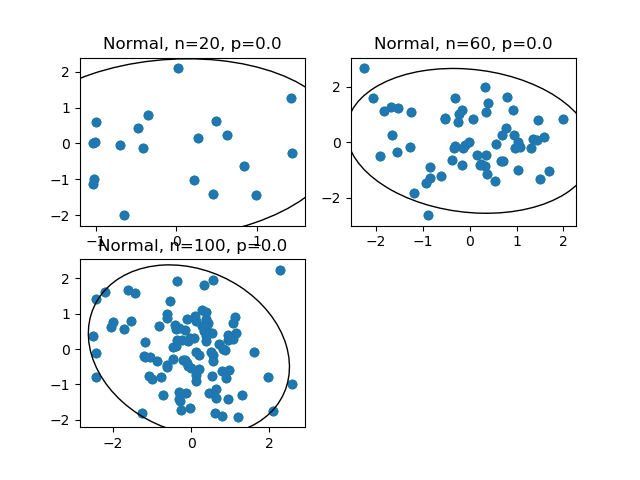
\includegraphics[width=\textwidth]{Normal0.png} 
				\caption[Двумерное нормальное распределение, при $\rho$ = 0]{Двумерное нормальное распределение, при $\rho$ = 0}
			\end{figure}
			\newpage
			\begin{figure}[h!]
				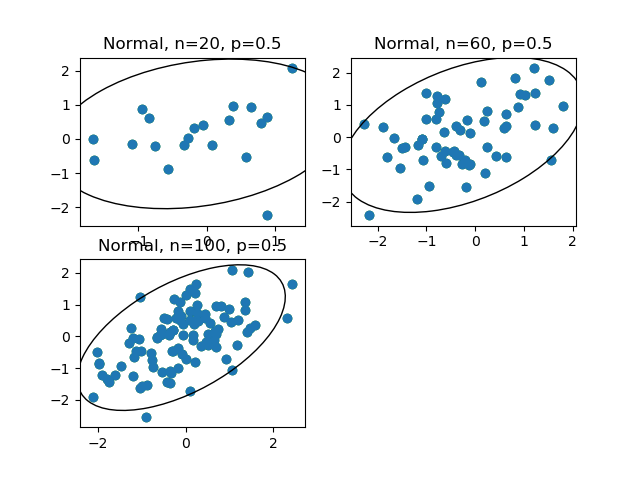
\includegraphics[width=\textwidth]{Normal5.png} 
				\caption[Двумерное нормальное распределение, при $\rho$ = 0.5]{Двумерное нормальное распределение, при $\rho$ = 0.5}
			\end{figure}
			\newpage
			\begin{figure}[h!]
				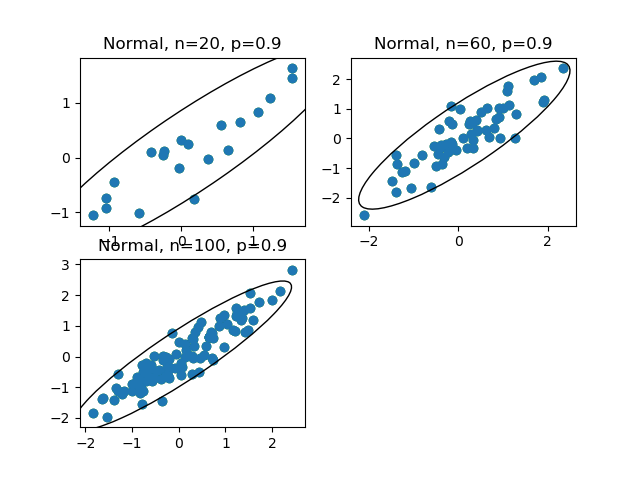
\includegraphics[width=\textwidth]{Normal9.png} 
				\caption[Двумерное нормальное распределение, при $\rho$ = 0.9]{Двумерное нормальное распределение, при $\rho$ = 0.9}
			\end{figure}
			\newpage
			\begin{figure}[h!]
				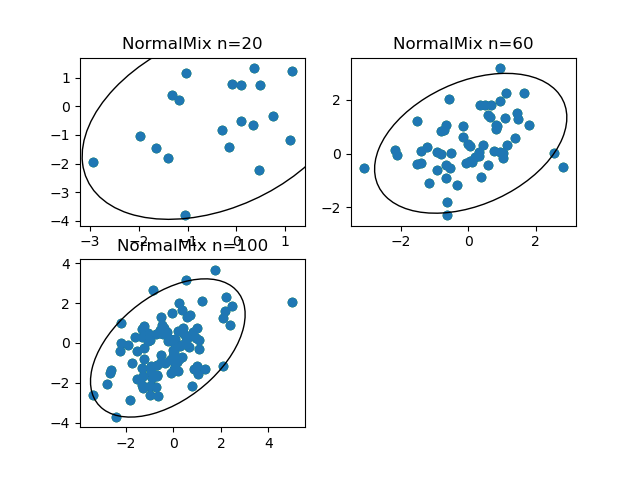
\includegraphics[width=\textwidth]{NormalMix9.png} 
				\caption[Смесь нормальных распределений]{Смесь нормальных распределений}
			\end{figure}
			
		\end{center}
		
		\subsection{Графики линейной регрессии}
		\begin{figure}[h!]
			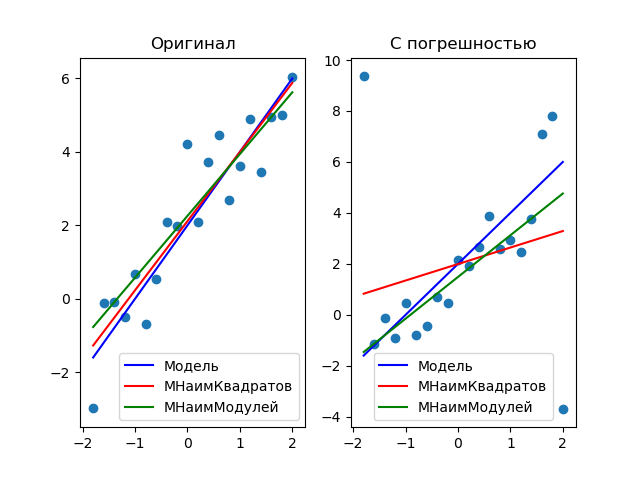
\includegraphics[width=\textwidth]{Graph.png} 
			\caption[Графики линейной регрессии при выборке с возмущением и без]{Графики линейной регрессии при выборке с возмущением и без}
		\end{figure}
		
		\subsection{Выборка без возмущений}
		Критерий наименьших квадратов:\\
		$$\hat{a} \approx 1.93,\hat{b} \approx 2.19$$\\
		
		Критерий наименьших модулей:\\
		$$\hat{a} \approx 2.24 ,\hat{b} \approx 1.77$$
		\subsection{Выборка с возмущниями}
		Критерий наименьших квадратов:\\
		$$\hat{a} \approx 0.48,\hat{b} \approx 1.76$$\\
		
		Критерий наименьших модулей:\\
		$$\hat{a} \approx 1.85 ,\hat{b} \approx 1.39$$
		\subsection{Метод максимального правдоподобия и $\chi^2$}
		Метод максимального правдоподобия:\\
		$$\hat{\mu} \approx 0.03, \hat{\sigma} \approx 0.95$$
		Критерий согласия $\chi^2$:
		\begin{table}[h!]
			
			\caption{Вычисление $\chi^2_B$ при проверке гипотизы $H_0$ о нормальном законе распределения N($x, \hat{\mu} \approx 0.16, \hat{\sigma} \approx 1.04$)}
			\label{tab:my_label}
			\begin{center}
				\vspace{5mm}
				
				\begin{tabular}{|c|c|c|c|c|c|c|}
					\hline
					i & $Delta_i$ , $a_{i - 1}$, $a_i$          &   $n_i$ &   $p_i$ &   $np_i$ &   $n_i-np_i$ &   $\frac{(n_i-np_i)^2}{np_i}$ \\
					\hline
					1 & [-$\infty$, -1.01] & 14 &  0.1562 &    15.62 &        -1.62 &        0.17 \\
					\hline
					2 & [-1.01, -0.37]     & 19 &  0.2004 &    20.04 &        -1.04 &            0.05 \\
					\hline
					3 & [-0.37, 0.28]      &  23 &  0.2517 &    25.17 &        -2.17 &               0.19 \\
					\hline
					4 & [0.28, 0.92]       &   19 &  0.2122 &    21.22 &        -2.22 &           0.23 \\
					\hline
					5 & [0.92, 1.56]       &  14 &  0.1201 &    12.01 &         1.99 &        0.33    \\
					\hline
					6 & [1.56, $\infty$]   & 11 &  0.0594 &     5.94 &         5.06 &         4.32 \\
					\hline
					$\sum$ & -                  &     100 &  1.0000      &   100.00    &         0.00  &                         5.29 = $\chi^2_B$\\
					\hline
				\end{tabular}
			\end{center}
		\end{table}
		
		Количество промежутков k = 6.\\
		Уровень значимости $\alpha$ = 0.05.\\
		
		\subsection{Доверительные интервалы}
		
		\begin{table}[h!]
			
			\caption{Доверительные интервалы для параметров нормального распределения}
			\label{tab:my_label}
			\begin{center}
				\vspace{5mm}
				
				\begin{tabular}{|c|c|c|}
					\hline
					n = 20 & m & $\sigma$\\
					\hline
					& -0.48 < m < 0.54 & 0.83 < $\sigma$ < 1.59\\ 
					\hline
					& &\\
					\hline
					n = 100 & m & $\sigma$\\
					\hline
					& -0.25 < m < 0.15 & 0.9 < $\sigma$ < 1.19\\
					\hline
				\end{tabular}
			\end{center}
		\end{table}
		
		\begin{table}[h!]
			
			\caption{Доверительные интервалы для параметров произвольного распределения. Асимптотический подход}
			\label{tab:my_label}
			\begin{center}
				\vspace{5mm}
				
				\begin{tabular}{|c|c|c|}
					\hline
					n = 20 & m & $\sigma$\\
					\hline
					& -0.43 < m < 0.49 & 0.93 < $\sigma$ < 1.25\\ 
					\hline
					& & \\
					\hline
					n = 100 & m & $\sigma$\\
					\hline
					& -0.25 < m < 0.15 & 0.95 < $\sigma$ < 1.09\\
					\hline
				\end{tabular}
			\end{center}
		\end{table}
		
		
		
	\section{Обсуждение}
		\subsection{Выборочные коэффициенты корреляции и эллипсы рассеивания}
			1)Сравним дисперсии выборочных коэффициентов корреляции.\\
			– Для двумерного нормального распределения дисперсии выборочных коэффициентов корреляции упорядочены следующим образом: r < $r_S$ < $r_Q$.\\
			– Для смеси нормальных распределений дисперсии выборочных
			коэффициентов корреляции упорядочены следующим образом:
			$r_Q$ < $r_S$ < r.\\
			
			2)Процент попавших элементов выборки в эллипс рассеивания ($95\%$-я доверительная область) примерно равен его теоретическому значению ($95\%$). При малом количестве событий <$\approx$ 12  Процент попавших элементов в эллипс рассеивания примерно равен 100$\%$.
		\subsection{Стравнение с теоретическими данными}
		По таблицам видно, что при увеличении объёма выборки, подсчитанные коэффициенты стремятся к теоретическим.\\
		По графикам видно, что при уменьшении корреляции эллипс равновероятности стремится к окружности, а при увеличении растягивается.
		\subsection{МНК и МНМ}
		1)МНК оценивает коэффициенты линейной регрессии точнее, на выборке без возмущений.\\
		Для доказательства этого введём метрику суммы квадратов разностей значений по оси y между МНК и модели и МНМ и модели. $\rho_1$ = $\sum (y_{MNK} - y_{etl})^2$ , $\rho_2$ = $\sum (y_{MNM} - y_{etl})^2$ и увидим, что $\rho_1$ всегда меньше $\rho_2$.\\ 
		\begin{center}
			Пример: \\
			$y_{etl}$ = [-1.60, -1.20, -0.80, -0.40,  0.00,   0.40,  0.80, 1.20,  1.60,  2.00,   2.40,  2.80,  3.20,  3.60, 4.00,  4.40,  4.80,  5.20,  5.60,  6.0 ]\\
			$y_{MNK} \approx $ [-1.27, -0.89, -0.52,  -0.14,  0.23,  0.61, 0.98,  1.36,  1.74,  2.11,  2.491,  2.86, 3.24,  3.62  3.99   4.37,  4.75, 5.12, 5.50  5.85]\\
			$y_{MNM} \approx$ [-0.77, -0.43, -0.09,  0.23,  0.57,  0.911,  1.24,  1.58,  1.92,  2.25,  2.59,  2.93,  3.26,  3.60,  3.94,  4.27,  4.61,  4.95,  5.28,  5.62]\\
			
			МНК : $\hat{a}$ = 1.88, $\hat{b}$ = 2.11\\
			МНМ : $\hat{a}$ = 2.26, $\hat{b}$ = 1.68\\
			
			$\rho_1$ = 16.59\\
			$\rho_2$ = 17.96\\
			
			Таким образом, $\rho_1$ < $\rho_2$.
		\end{center}
		
		2)На выборке с возмущениями эффективнее использовать МНМ. Таким образом, метод наименьших модулей устойчив к редким выбросам, в свою очередь МНМ обладает большей сложностью вычислений, чем МНК(т.к. ,в коде, МНК - оценки вычисляются из расчётных формул, а МНМ - оценки вычисляются, через решение задачи минимизации).
		
		
		\subsection{Критерий Пирсона}
			По результатам работы, значение критерия согласия Пирсона:\\
			$\chi^2_B = 5.29$. Табличное значение квартиля $\chi^2_{1 - \alpha}(k - 1) = \chi^2_{0.95}(5) = 11.07$.\\
			
			Таким образом, $\chi^2_B < \chi^2_{0.95}(5)$, из этого следует, что основная гипотеза $H_0$(о нормальном законе распределения N($x, \hat{\mu}, \hat{\sigma}$)), на уровне зависимости $\alpha$ = 0.05, соотносится с выборкой.
			
			При распределении Лапласа(n = 30), $$\hat{\mu} \approx 0.53, \hat{\sigma} \approx 1.52$$\\
			По результатам работы, значение критерия согласия Пирсона:\\
			$\chi^2_B = 12.94$.\\
			Таким образом, $\chi^2_B > \chi^2_{0.95}(5)$, из этого следует, что основная гипотеза $H_0$(о нормальном законе распределения N($x, \hat{\mu}, \hat{\sigma}$)), на уровне зависимости $\alpha$ = 0.05, при распределении Лапласа не верна.
		
		\subsection{Доверительные интервалы}
			Генеральные характеристики m = 0, $\sigma$ = 0 накрываются построенными доверительными интервалами.\\
			
			По полученным результатам видно, что лучший результат достигается на выборках большого объема.\\
			При сравнении результатов при объеме n = 20, видим, что интервал меньше для парамаетров произвольного распределения.
	\section{Литература}
	
	\href{https://physics.susu.ru/vorontsov/language/numpy.html}{Модуль numpy}\\
	
	\href{https://matplotlib.org/}{Модуль matplotlib}\\
	
	\href{https://www.scipy.org/}{Модуль scipy}\\
	
	
	\href{https://ru.wikipedia.org/wiki/%D0%9C%D0%BD%D0%BE%D0%B3%D0%BE%D0%BC%D0%B5%D1%80%D0%BD%D0%BE%D0%B5_%D0%BD%D0%BE%D1%80%D0%BC%D0%B0%D0%BB%D1%8C%D0%BD%D0%BE%D0%B5_%D1%80%D0%B0%D1%81%D0%BF%D1%80%D0%B5%D0%B4%D0%B5%D0%BB%D0%B5%D0%BD%D0%B8%D0%B5}{Многомерное нормальное распределение}
	
	\href{https://ru.wikipedia.org/wiki/%D0%9A%D0%BE%D1%80%D1%80%D0%B5%D0%BB%D1%8F%D1%86%D0%B8%D1%8F}{Корреляция}
	
	\href{https://ru.wikipedia.org/wiki/%D0%9C%D0%B5%D1%82%D0%BE%D0%B4_%D0%BD%D0%B0%D0%B8%D0%BC%D0%B5%D0%BD%D1%8C%D1%88%D0%B8%D1%85_%D0%BC%D0%BE%D0%B4%D1%83%D0%BB%D0%B5%D0%B9}{Метод наименьших модулей}\\
		
	\href{https://ru.wikipedia.org/wiki/%D0%9C%D0%B5%D1%82%D0%BE%D0%B4_%D0%BD%D0%B0%D0%B8%D0%BC%D0%B5%D0%BD%D1%8C%D1%88%D0%B8%D1%85_%D0%BA%D0%B2%D0%B0%D0%B4%D1%80%D0%B0%D1%82%D0%BE%D0%B2}{Метод наименьших квадратов}\\
	
	\href{https://ru.wikipedia.org/wiki/%D0%9A%D0%B2%D0%B0%D0%BD%D1%82%D0%B8%D0%BB%D0%B8_%D1%80%D0%B0%D1%81%D0%BF%D1%80%D0%B5%D0%B4%D0%B5%D0%BB%D0%B5%D0%BD%D0%B8%D1%8F_%D1%85%D0%B8-%D0%BA%D0%B2%D0%B0%D0%B4%D1%80%D0%B0%D1%82}{Таблица значений $\chi^2$}\\
		
	\href{https://ru.wikipedia.org/wiki/%D0%9D%D0%BE%D1%80%D0%BC%D0%B0%D0%BB%D1%8C%D0%BD%D0%BE%D0%B5_%D1%80%D0%B0%D1%81%D0%BF%D1%80%D0%B5%D0%B4%D0%B5%D0%BB%D0%B5%D0%BD%D0%B8%D0%B5}{Нормальное распределение}\\
		
	\href{http://mit.spbau.ru/sewiki/images/a/a1/Cis.pdf}{Доверительные интервалы}\\
	
	\section{Приложения}
	
	\href{https://github.com/LuciusGen/Matstat/blob/master/Lab5/Lab5.py}{Код 5-й лаборатрной}
	
	\href{https://github.com/LuciusGen/Matstat/blob/master/Lab5/lab5.tex}{Код 5-о отчёта}
	
	\href{https://github.com/LuciusGen/Matstat/blob/master/Lab6/Lab6.py}{Код 6-й лаборатрной}
	
	\href{https://github.com/LuciusGen/Matstat/blob/master/Lab6/lab6.tex}{Код 6-о отчёта}
	
	\href{https://github.com/LuciusGen/Matstat/blob/master/Lab6/Lab7.py}{Код 7-й лаборатрной}
	
	\href{https://github.com/LuciusGen/Matstat/blob/master/Lab6/lab7.tex}{Код 7-о отчёта}
	
	\href{https://github.com/LuciusGen/Matstat/blob/master/Lab8/Lab8.py}{Код 8-й лаборатрной}
	
	\href{https://github.com/LuciusGen/Matstat/blob/master/Lab8/lab8.tex}{Код 8-о отчёта}
	
\end{document}